
\section[Salem--Schaeffer measures]{Salem--Schaeffer measures}

%\subsection{}

\def\B{\mathscr{B}}
\def\Alg{\mathscr{A}}
\def\Mes{\mathscr{M}}
\def\Rajch{\mathscr{R}}
\def\W{\mathscr{W}}
\def\L{\mathscr{L}}
\def\T{\Hat T}
\def\CL{{\mathrm{CL}}}

%=================================================================================================
\begin{frame}
\begin{center}
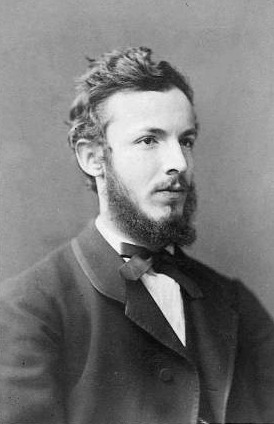
\includegraphics[height=36mm]{Georg_Cantor3.jpg}

Georg Cantor


\bigskip
\bigskip

\includegraphics[width=98mm]{CantorSet.pdf}

$\cK$

\end{center}
\end{frame}


%=================================================================================================
\begin{frame}
\begin{center}

\includegraphics[width=72mm]{CantorSet_1.pdf}

\end{center}
\end{frame}


%=================================================================================================
\begin{frame}
\begin{center}

\includegraphics[width=72mm]{CantorSet_2.pdf}

\end{center}
\end{frame}


%=================================================================================================
\begin{frame}
\begin{center}

\includegraphics[width=72mm]{CantorSet_3.pdf}

\end{center}
\end{frame}


%=================================================================================================
\begin{frame}
\begin{center}

\includegraphics[width=72mm]{K2.pdf}

\end{center}
\end{frame}


%=================================================================================================
\begin{frame}
\begin{center}

\includegraphics[width=72mm]{K2L.pdf}

\end{center}
\end{frame}


%=================================================================================================
\begin{frame}
\begin{center}

\visible<2>{
$\mu_{\CL} \conv \mu_{\CL}$

\includegraphics[width=77mm]{KconvK.pdf}$\;$
}

\bigskip

\includegraphics[width=72mm]{KplusK.pdf}

$\cK+\cK = [0,2]$

\end{center}
\end{frame}


\if0=1
%=================================================================================================
\begin{frame}

{\bf Definition.} 
$\mu \conv \nu$ is the distribution of the sum $x+y \pmod{1}$ 
of a $\mu$-distributed $x$ and a $\nu$-distributed $y$,
$$
  \mu \conv \nu(C) = \iint_{\{(x,y)\in\Set{T}^2 \where x+y \in C\}} 1 \,d\mu(x) \,d\nu(y), 
$$
where $\Set{T} = \Set{R}/\Set{Z}$. 

\bigskip
\visible<2>{
{\bf Construction.} An example of spectral measure 

\includegraphics[width=36mm]{CantorSet.pdf} $\quad$
\includegraphics[width=20mm]{K2s.pdf} $\quad$
\includegraphics[width=15mm]{K3.pdf} $\qquad$ $\dots$

$\sigma = \mu_{\CL} + \qquad \qquad \qquad \quad 
      {\small \frac12}\mu_{\CL}\conv\mu_{\CL} + \quad 
      {\small \frac14}\mu_{\CL}\conv\mu_{\CL}\conv\mu_{\CL} + \quad \dots$ 
}

\end{frame}
\fi


%=================================================================================================
\begin{frame}
  \frametitle{Notation}

  Let $\Mes([0,1)) = \Mes$ be the set of Borel measures on $\Set{T}$.

  \bigskip
  Recall that $\nu \ll \mu$ if $\nu = p(x)\mu$, where $p \in L^1(\mu)$.

  \bigskip
  We say that $\nu \perp \mu$ if $\nu(E) = \mu(E^c) = 1$ for an $E \in \B$.

  \bigskip
  {\it Observation}. For any $\mu \in \Mes$
  $$
    \mu = \mu_d + \mu_s + \mu_{ac}, 
  $$
  where $\mu_d = \sum_j b_j \df_{x_j}$, $\mu_s \perp \la$ is purely singular, 
  and $\mu_{ac} \ll \la$, where $\la$ is Lebesgue measure. 

\end{frame}


%=================================================================================================
\begin{frame}
  \frametitle{Harmonic analysis}

  Fourier coefficients of a measure $\mu$, 
  $$
    \Hat\mu(n) = \int e^{-2\pi i\, nx} \,d\mu(x).  
  $$
  
  \pause
  \bigskip
  {\bf Self-similarity phenomenon.} %\\ 
  $$\cK = 3\cK$$ %$\impl\quad $
  Thus, Cantor--Lebesgue measure $\mu_{\CL}$ satisfies 
  $$
    \Hat\mu_{\CL}(n) = \Hat\mu_{\CL}(3n) = \dots = \Hat\mu_{\CL}(3^k n) = \dots
  $$
  
\end{frame}


%=================================================================================================
\begin{frame}
  \frametitle{Menshov--Rajchman measures}

  \begin{center}
  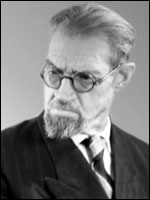
\includegraphics[height=30mm]{Menshov_DE}
  
  Dmitrii Menshov
  \end{center}

  {\bf Definition.} A measure $\mu$ is called {\it Menshov--Rajchman\/} if
  $$
    \Hat\mu(n) \to 0 \qquad \text{as $n \to \infty$}
  $$
  Let $\Rajch$ be the class of such measures.
  
\end{frame}


%=================================================================================================
\begin{frame}
  \frametitle{Riemann--Lebesgue theorem}

  \begin{center}
  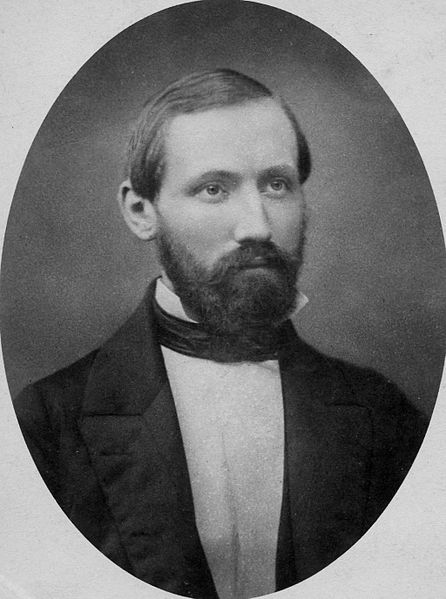
\includegraphics[height=30mm]{446px-Bernhard_Riemann_2.jpg} $\quad \qquad$
  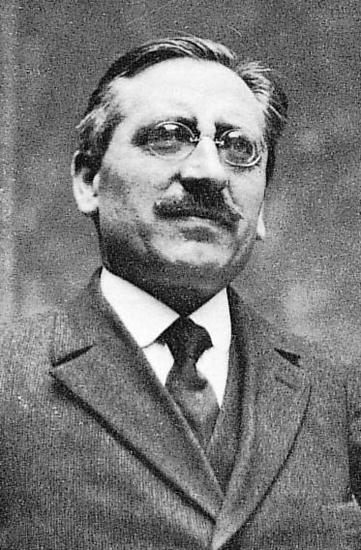
\includegraphics[height=30mm]{Lebesgue2.jpg}
  
  $\quad$ Bernhard Riemann $\quad$ Henri L\'eon Lebesgue
  \end{center}
  
  \bigskip
  \bigskip

  
  {\bf Theorem} (Riemann--Lebesgue). If $\mu \ll \la$ then $\mu \in \Rajch$. 
  
  \bigskip
  \bigskip
  \bigskip
  
\end{frame}


%=================================================================================================
\begin{frame}
  \frametitle{Menshov--Rajchman measures}

  \begin{columns}[t]
    \begin{column}{0.4\textwidth}
      \begin{center}
      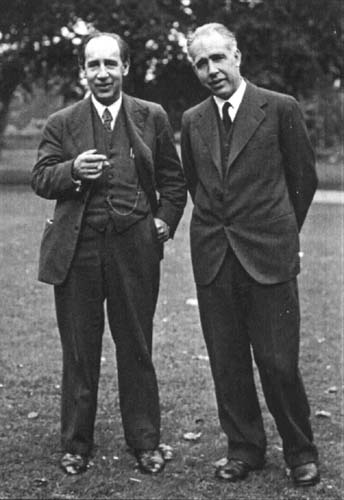
\includegraphics[height=54mm]{Bohrs.jpeg}
      
      Harald and Niels Bohr 
      \end{center}
    \end{column}
    \begin{column}{0.6\textwidth} 
  
      {\it Observation}.
      If $\mu_d$ is discrete then $\Hat\mu_d(n)$ is Bohr almost periodic, and $\mu$ is never Rajchman.

      \bigskip
      {\it Observation}. $\Hat\mu_\CL(3n) = \Hat\mu_\CL(n)$, hence, $\mu_\CL \not\in \Rajch$.
      
      \bigskip
      {\bf Theorem} (Menshov, 1916). \\ 
      There exists a singular $\mu \in \Rajch$. 

    \end{column}
  \end{columns}
    
\end{frame}


%=================================================================================================
\begin{frame}
  \frametitle{Dynamical system interpretation}

  Let $T$ be an invertible measure preserving transformation of a~Borel probability space $(X,\Alg,\eta)$.
  The {\it Koopman operator\/}  
  $$\Hat T \Maps L^2(\mu) \to L^2(\mu) \Maps f(x) \mapsto f(Tx).$$
  
  \bigskip
  {\bf Definition.} Spectral measure $\mu_f$ is defined by the equation
  $$
    \Hat\sigma_f(-n) = \int_{S^1} z^n \,d\mu_f = \langle \Hat T^n f,f \rangle.
  $$
  
  %\pause
  \medskip
  {\it Remark}.
  In dynamical system language: 
  $$
    \sigma_f \text{ is Rajchman} \quad \iff \quad \sigma_f \text{ is {\it mixing}.}
  $$
  
\end{frame}



  %{\bf Theorem} (Neder, 1920). % \\ 
  %A Rajchman measure cannot be a~combination of discrete and continuous measures.

%=================================================================================================
\begin{frame}
  \frametitle{Weak mixing}

  \begin{center}
  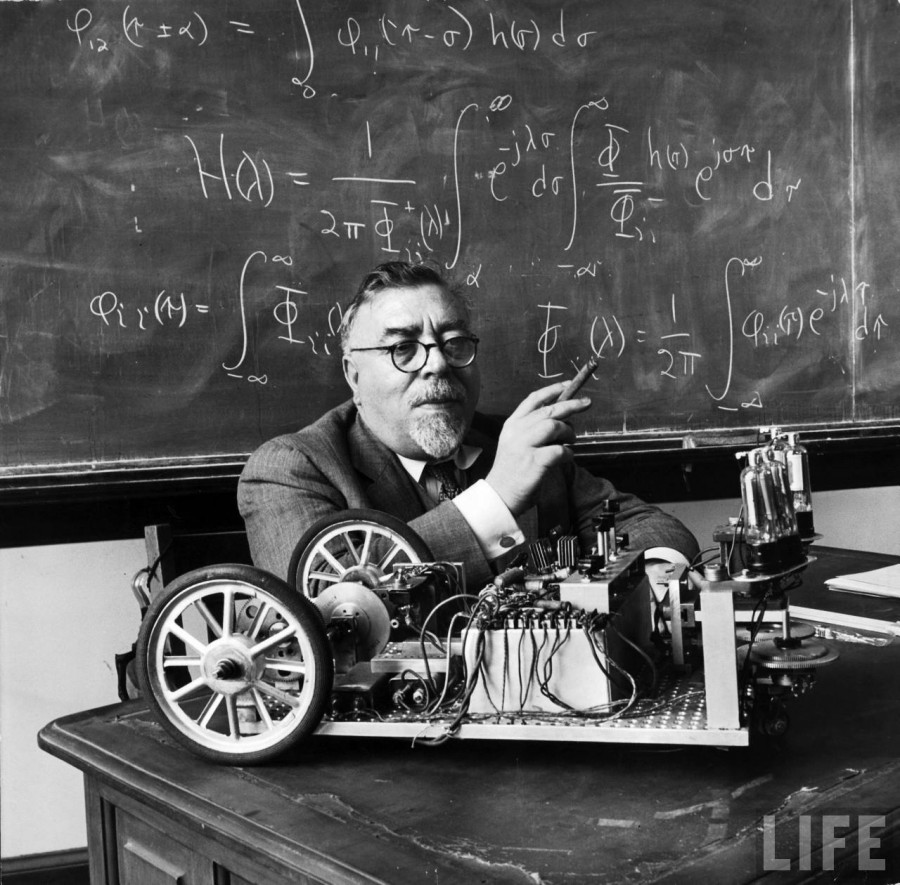
\includegraphics[height=36mm]{NorbertWiener.jpg}
  
  Norbert Wiener
  \end{center}
  
  \bigskip
  {\bf Theorem} (Wiener, 1924). % \\ 
  If $\mu$ is continuous then for any $\eps > 0$ 
  $$
    \mathrm{density}\{n \where |\Hat\mu(n)| > \eps\} = 0. 
  $$
  
  %\pause
  %\bigskip
  %{\it Remark}. $T$ is called {\it weakly mixing\/} $\iff$ all $\mu_f$ are continuous. 
    
\end{frame}


%=================================================================================================
\begin{frame}
  \frametitle{Polynomial decay of $\Hat\mu(n)$}

  \begin{center}
  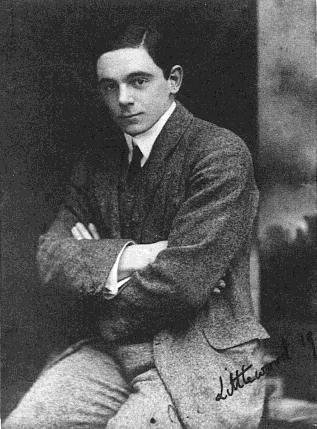
\includegraphics[height=36mm]{Littlewood.png}
  
  John Littlewood
  \end{center}

  \bigskip
  {\bf Theorem} (Littlewood, 1936). % \\ 
  There exists a singular measure $\mu$ such~that $\Hat\mu(n) = O(|n|^{-c})$ with $c > 0$.
  
  \bigskip
    
\end{frame}


%=================================================================================================
\begin{frame}
  \frametitle{Salem--Schaeffer measures}
  
  {\bf Theorem} (Wiener, Wintner, 1938). The constant $c$ can be arbitrarily close to~$1/2$.   
  
  %\pause
  \bigskip
  {\it Note\/}: if $c > 1/2$ then $\Hat\mu \in L^2(\Set{Z})$ and $\mu \ll \la$. 
  
  %\pause
  \bigskip
  {\bf Theorem} (Schaeffer, 1939). There exist singular measures $\mu$ with 
  $$
    \Hat\mu(n) = O\bigl(r(|n|) \cdot |n|^{-1/2}\bigl) 
  $$
  for any increasing sequence $r(n) \to \infty$.
  
  %\bigskip
  %The method: generalized Riesz products. 
  
  %\pause
  \bigskip
  Futher progress will be achieved by Salem (1943--44), Ivashev-Musatov (1956) et al. 
  
\end{frame}


%=================================================================================================
\begin{frame}
  \frametitle{Salem--Schaeffer measures}
  
  \begin{center}
  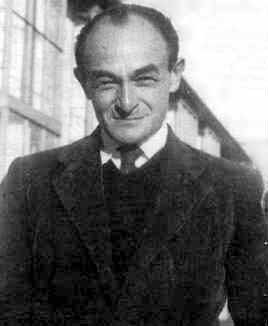
\includegraphics[height=30mm]{salem.jpg}
  
  Rapha\"el Salem
  \end{center}
  
  \bigskip
  {\bf Definition.} $\mu$ is a {\it Salem--Schaeffer\/} measure if $\kappa(\mu) = -1/2$, 
  $$
    \kappa(\mu) = \inf\{ \gamma \where \Hat\mu(n) = O(|n|^{\gamma}) \}. 
  $$

\end{frame}


%=================================================================================================
\begin{frame}
  \frametitle{Salem--Schaeffer measures}

  {\bf Questions.} 
  
  \begin{itemize}
   \item Dynamical system models for Salem--Schaeffer measures? \\[9pt]
   \item Ergodic properties of systems with Salem spectral type? \\[9pt]
   \item Interpretation of self-similarity effects?
  \end{itemize}

  
\end{frame}



%=================================================================================================
\section{Dynamical system models}

\begin{frame}
  \frametitle{Dynamical system models}

  Our purpose is to construct spectral measures of Salem type.

  \bigskip
  {\bf Main construction.} \\
  Let $G$ be a Lie group or a discrete group. Consider a $G$-odometer
  $$
    G/\G_0 \stackrel{\pi_0}\longleftarrow \dots 
      \stackrel{\pi_{n-1}}\longleftarrow
    G/\G_n \stackrel{\pi_n}\longleftarrow
    G/\G_{n+1} \stackrel{\pi_{n+1}}\longleftarrow \dots
      \longleftarrow
    X_0.
  $$
  Further, for each lattice $\G_n < G$ 
  fix a fundamental domain $U_n$ %,   then represent 
  $$
    G/\G_{n+1} = \bigsqcup_{\gamma \in \G_n/\G_{n+1}} U_n\gamma \pmod{0} 
  $$
  
\end{frame}

\begin{frame}
  \frametitle{Dynamical system models}

  \dots And define arbitrarily 
  $$
    \phi_n \Maps G/\G_{n+1} \to G/\G_n, 
  $$
  such that given $x = a\G_{n+1} \in U_n\gamma$, we set 
  $$
    \phi_n(x) = L_{\alpha_{n,\gamma}} \mathbin{\circ} \pi_n(x), 
  $$
  where $L_g(a\G_n) = ga\G_n$, and the rotations $\alpha_{n,\gamma}$ are the 
  {\em parameters of the constructions}. In~other words, after projection onto $G/\G_n$ 
  each copy $U_n\gamma$ is rotated by~$\alpha_{n,\gamma}$. 
  
  \bigskip 
  {\it Observation.} The maps $\phi_n$ are generally discontinuous. 
  
\end{frame}

%\ifnum0=1
\begin{frame}
  \frametitle{Dynamical system models}

  % Our purpose is to construct spectral measures of Salem type.
  {\bf Illustration to the main construction for $G = \Set{Z}^2$}
  
  %\pause
  \bigskip
  We start with the original configuration $\W_0$ on $G/\G_0 \cong \Set{Z}_4^2$ 
  
  \begin{center}
   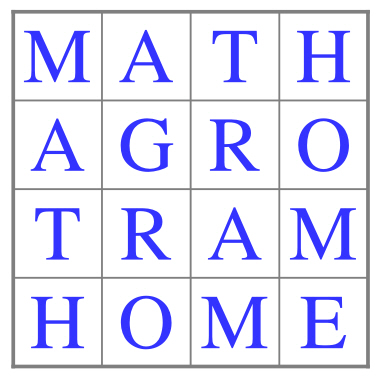
\includegraphics[height=33mm]{pic1.jpg}
  \end{center}
  
\end{frame}


%=================================================================================================
\begin{frame}
  \frametitle{Dynamical system models}
  
  {\footnotesize 
  Then we build the next configuration $\W_1$ on a~bigger homoeneous space 
  by applying a~random rotation on each copy of the configuration $\W_0$. }
  
  \begin{center}
   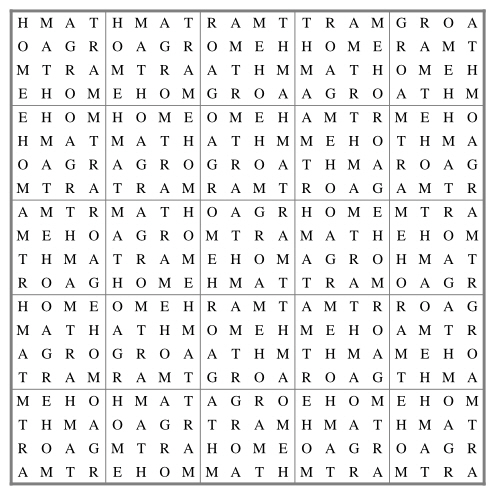
\includegraphics[height=58mm]{pic2.jpg}
  \end{center}
  
\end{frame}


%=================================================================================================
\begin{frame}
  \frametitle{Dynamical system models}
  
  {\footnotesize 
  Then we build the next configuration $\W_1$ on a~bigger homoeneous space 
  by applying a~random rotation on each copy of the configuration $\W_0$. }
  
  \begin{center}
   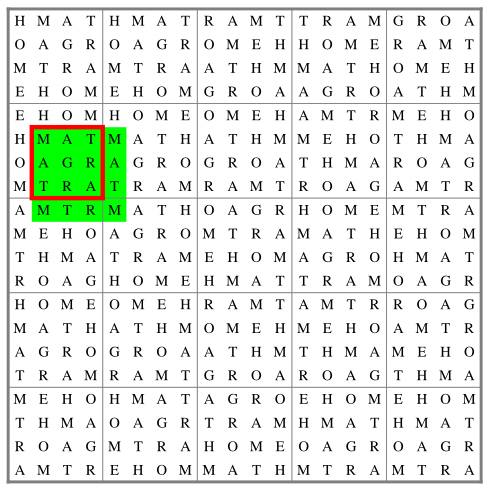
\includegraphics[height=57mm]{pic3.jpg}
  \end{center}
  
\end{frame}


%=================================================================================================
\begin{frame}
  \frametitle{Dynamical system models}
  
  Consider another sample configuration for $G = \Set{Z}_2$ and 
  $\G_1,\;\G_2,\;\ldots = 3\Set{Z}^2,\; 15\Set{Z}^2,\; \ldots$ 
  %
  We show $\W_n$ in different colouring. 
  
  \begin{center}
   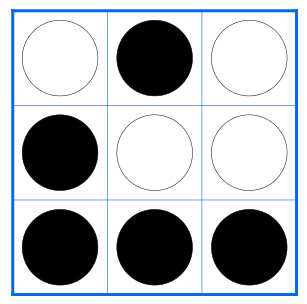
\includegraphics[height=36mm]{pic4.jpg}
  \end{center}
  
\end{frame}


%=================================================================================================
\begin{frame}
  \frametitle{Dynamical system models}
  
  \begin{center}
   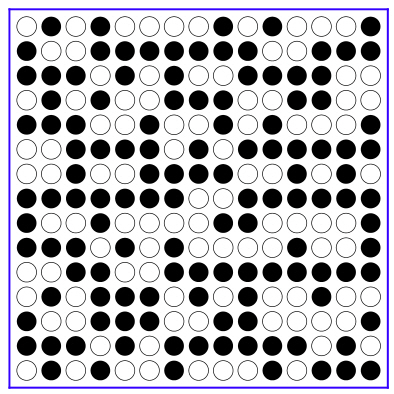
\includegraphics[height=64mm]{pic5.jpg}
  \end{center}
  
\end{frame}


%=================================================================================================
\begin{frame}
  \frametitle{Dynamical system models}
  
  \begin{center}
   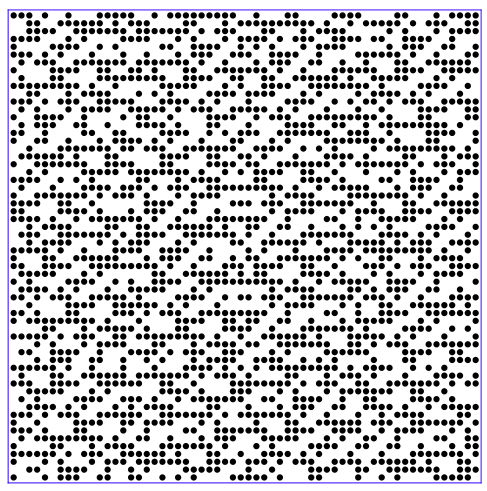
\includegraphics[height=64mm]{pic6.jpg}
  \end{center}
  
\end{frame}


%=================================================================================================
\begin{frame}
  \frametitle{Dynamical system models}
  
  \begin{center}
   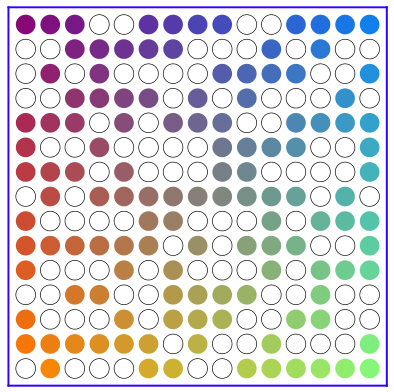
\includegraphics[height=64mm]{pic7.jpg}
  \end{center}
  
\end{frame}


%=================================================================================================
\begin{frame}
  \frametitle{Dynamical system models}
  
  \begin{center}
   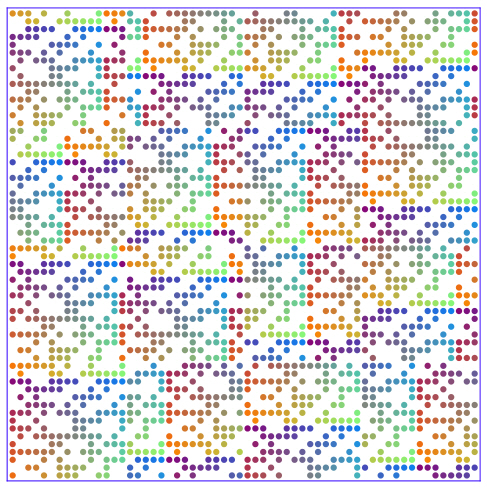
\includegraphics[height=64mm]{pic8.jpg}
  \end{center}
  
\end{frame}


%=================================================================================================
\begin{frame}
  \frametitle{Dynamical system models}
  
  \begin{center}
   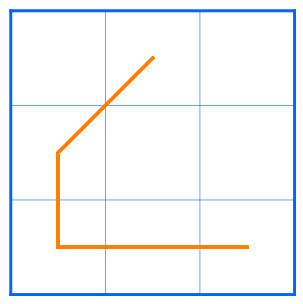
\includegraphics[height=36mm]{pic9.jpg}
  \end{center}
  
\end{frame}


%=================================================================================================
\begin{frame}
  \frametitle{Dynamical system models}
  
  \begin{center}
   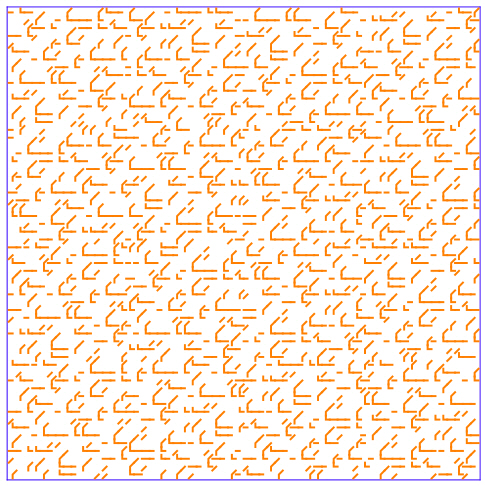
\includegraphics[height=64mm]{pic10.jpg}
  \end{center}
  
\end{frame}
%\fi


%=================================================================================================
\begin{frame}
  \frametitle{Salem measures of dynamical system origin: dimension~$1$}
  
  %{\bf Theorem} (A.P., 2009--13). There exist ergodic transformations having Salem spectral type and spectrum of multiplicity~$1$. 
  %
  %\bigskip
  %{\bf Theorem} (A.P.). There exist actions of groups $\Set{Z}^d$ and $\Set{R}^d$ having Salem spectral type. 

  %\bigskip
  %Ryzhikov, 2009--13: An alternative and simplier method for the case of transformation 
  %acting on an infinite measure space. 
  
  %Assume for simplicity that the one-dimensional construction is considered.
  
  Let $T$ be a transformation constructed above with i.i.d.\ random rotations,
  %\\ 
  and let $\sigma = \sigma_T$ be the spectral type of~$T$. % the action.
  
  \bigskip
  {\bf Theorem} -- Several properties of Salem-type constructions  
  \begin{itemize}
   \item $\sigma_f$ are Salem for a dense set of cylindric functions 
   \item in particular, $\sigma \conv \sigma \ll \lambda$
   \item $T$ has simple spectrum
   \item local rank $\beta(T) \ge 1/4$ $\impl$ $T$ has zero entropy 
   \item symbolic complexity $p_{w_\infty}(\ell) \sim \ell^3$ in a $\log$-scale 
  \end{itemize}

\end{frame}


\def\actionT{{\boldsymbol T}}

%=================================================================================================
\begin{frame}
  \frametitle{Salem measures of dynamical system origin: dimension~$2$}
  
  Now let $\actionT$ be an action of the group $\Set{Z}^2$, 
  given by random rotations of rectangular configurations, 
  and $\sigma = \sigma_\actionT$. 

  \bigskip
  {\bf Theorem} 
  \begin{itemize}
   \item $\actionT$ has zero entropy  
   \item $\sigma$ is Salem, in particularly, $\sigma \conv \sigma \ll \lambda$
   \item projection to any line $\pi_L \sigma \ll \lambda$
   \item $T$ has simple spectrum
   \item each $T^{(i,j)}$ has countable Lebesgue spectrum, but zero entropy 
  \end{itemize}

\end{frame}


%=================================================================================================
\begin{frame}
  \frametitle{Salem measures of dynamical system origin}

  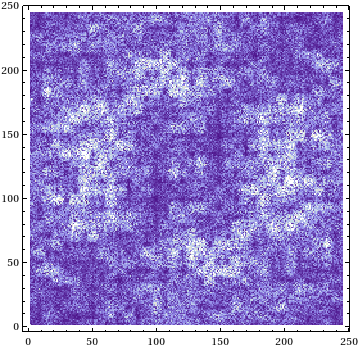
\includegraphics[height=43mm]{SpMeasIceberg2d_2.png} $\qquad $
  %
  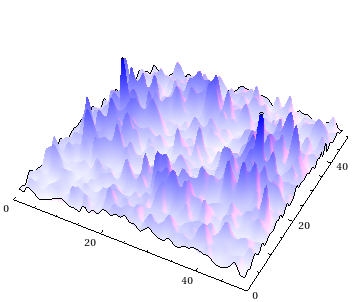
\includegraphics[height=43mm]{SpMeasIceberg2d_1.png}
  
\end{frame}


%=================================================================================================
\begin{frame}
  \frametitle{Scaled approximation and complexity}

  {\bf Definition A.} A trandformation $T$ on a Borel probability space $X$ 
  admits {\it approximation of type}~$\cI$ if $\forall\; \eps > 0$ and any measurable finite partition $\cP$ 
  there exist $X_\eps$ and a word $W_\eps$ such that for any point $x \in X_\eps$ 
  the code of $x$ is $\eps$-covered by rotations of~$W_\eps$. 
  
  \bigskip
  {\bf Definition B.} $T$ admits $\varphi$-scaled approximation if 
  in the scope of definition~A the code of $x$ is $\eps$-covered by subwords $w_j$ of $W_\eps$ 
  in such a way that the mean length $L(x)$ of $w_j$ exists and satisfies 
  $$
    L(x) \ge \varphi(|W_\eps|) \cdot |W_\eps|. 
  $$
  
\end{frame}


%=================================================================================================
\begin{frame}
  \frametitle{Easy and hard questions}
  
  {\bf Proposition.} Our Salem constructions (in dumension one) satisfy 
  scaled approximation with $\phi(\ell) = 1/2$. 

  \bigskip
  {\bf Definition.} Let 
  $$
    \kappa(T) = \inf\{ \gamma \where \kappa(\sigma_f) \le \gamma \quad \text{for $f$ in a dense set ${\mathcal F}$} \}
  $$
  
  \bigskip 
  {\bf Question.} Is it true that $\phi$-scaled approximation with $\phi(\ell) = c_0$ 
  implies that 
  $$
    \sup \{\kappa(f) \where f \in {\mathcal F} \} \ge -1/2
  $$
  for any dense set ${\mathcal F}$ of ``cylindric'' functions? 
\end{frame}



%=================================================================================================
%\section{Spectral self-similarity}
 %
%\begin{frame}
%  \frametitle{Dynamical system interpretation}
%  
%  {\bf Questions.} 
%  \begin{itemize}
%   \item Can we see the effects of spectral self-similarity for spectral measures of ergodic dynamical systems?
%   \item Can we found symmetries for Salem measures? 
%   \item How to interpret that symmetries in terms of the underlying system?
%  \end{itemize}
%  
%\end{frame}


\begin{frame}
  \frametitle{An example of self-similarity}
  
  Chacon's substitution system:

  \begin{flushright}
  \includegraphics[height=54mm]{Ch3Sta.pdf}
  \end{flushright}

  
\end{frame}


\begin{frame}
  \frametitle{An example of self-similarity}
  
  Let $T$ be the map associated with Chacon's substitution.
  
  Set $h_n = \frac{3^n-1}2$. 

  \bigskip
  {\bf Theorem} (E.Janvresse, T. de la Rue, A.P., V.Ryzhikov, '13). \\ 
  $\Hat T^{mh_n} \wto P_m(\T)$ and the semigroup 
  $$
    \L = \overline{\{\T^k \where k \in \Set{Z}\}} = \{P_{m_1}(\T)\cdots P_{m_r}(\T)\T^s,\ \Theta\},
  $$
  where $\Theta$ is the orthoprojector to contants. 
  
  \bigskip
  \begin{itemize}
   \item $P_m$ are self reciprocal
   \item Lee--Yang property: all roots of $P_m$ are real
   \item the family $P_m$ contains many irreducible polynomials
  \end{itemize}

\end{frame}


\begin{frame}
  \frametitle{Some misterious properties of polynomials $P_m$}

  Lee--Yang property (in dual coordinates)
  
  \begin{center}
  \includegraphics[height=48mm]{Ch3Roots122A.pdf}
  \end{center}
  
\end{frame}



\newcommand*{\threesim}{%
\mathrel{\vcenter{\offinterlineskip
\hbox{$\sim$}\vskip-.35ex\hbox{$\sim$}\vskip-.35ex\hbox{$\sim$}}}}

\begin{frame}
  \frametitle{An example of self-similarity}

  Let $\mu$ be a spectral measure of $T$.
  
  \bigskip
  {\it Observation}. $\mu(dx) \threesim \mu(3dx)$ -- weakly almost self-similar near $0$. % \stackrel\approx\sim
  
  \pause
  \bigskip
  {\it A stronger form of self-similarity}. \\ 
  The family $P_m$ is a fixed point of a random walk on a Shreier graph $BS(1,3)/\langle \sigma \rangle$ of the group 
  $$
    BS(1,3) = \langle \sigma, a \: \mid \: \sigma a\sigma^{-1} = a^3 \rangle 
  $$
  %
  acting naturally on $\Set{Q}_{(3)}$ by 
  $$
    \sigma \Maps x \mapsto 3x, \qquad x \mapsto x+1. 
  $$
  % 
  % Here the hyperbolic element corresponds to $\sigma \Maps z \mapsto z^3$

\end{frame}


\begin{frame}
  \frametitle{Extending self-similarity properties}

  Cayley graph of $BS(1,3)$

  \begin{center}
  $\quad$ \includegraphics[height=48mm]{pic51.pdf}
  \end{center}

\end{frame}


\begin{frame}
  \frametitle{Extending self-similarity properties}

  Cayley graph of $BS(1,3)$

  \begin{center}
  \includegraphics[height=48mm]{pic52.pdf}
  \end{center}

\end{frame}


%=================================================================================================
\begin{frame}
  \frametitle{Pascal adic transformation}
  
  \begin{center}
    \includegraphics[height=55mm]{PascalAdic.pdf}

    Bratelli--Vershik diagram of {\it Pascal adic transformation\/} $T_V$ 
  \end{center}
  
\end{frame}


%=================================================================================================
\begin{frame}
  \frametitle{Pascal adic transformation}
  
  \begin{center}
    \includegraphics[height=58mm]{PascalAdicTowers2.pdf}

    {\small Cutting and stacking representation of the Pascal adic map ($n = 8$)}  
  \end{center}
  
\end{frame}



%=================================================================================================
\begin{frame}
  \frametitle{Pascal adic transformation}
  
  \begin{center}
    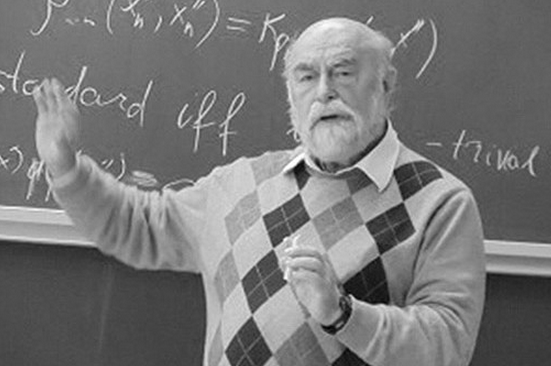
\includegraphics[height=28mm]{Vershik2.png}
  \end{center}

  \medskip
  Several remarkable properties of Pascal adic transformation:
  \begin{itemize}
    \item $T_V$ is ergodic and has zero entropy
    \item symbolic complexity $p_{w_\infty}(\ell) \sim \frac16 \ell^3$
    \item $T_V$ admits $\varphi$-scaled approximation with $\varphi(\ell) \sim c_1 \log^{-1/2} \ell$ 
    \item ${}^{***}$ self-similarity properties described in terms of {\color{red} $BS(1,2)$}  
  \end{itemize}
  
  \bigskip
 
\end{frame}



%=================================================================================================
\begin{frame}
  \frametitle{Easy and hard questions}
  
  {\bf Questions.} 
  \begin{itemize}
   \item $T_V$ is mixing? 
   \item $\kappa(\sigma_f) \ge -1/2$ for any cylindric function $f \;$?
  \end{itemize}
  
  \bigskip
  {\bf Question.} 
  Is it true that both Vershik's map $T_V$ and Salem-type constructions have \underline{infinite}\ rank? 
  % (cannot be approximated by a sequence of $m$-tuples of Rokhin towers) 
  
  \bigskip
  {\bf Question.} 
  Find in a class of systems having Salem spectral type 
  two systems which are spectrally equivalent but not conjugate.  
  
  %\bigskip
  %{\bf Question.} 
  %Study the geometry of spectral measures for Salem constructions
  
  
\end{frame}


%***********************************8
\section{Proofs}

%=================================================================================================
\begin{frame}
  \frametitle{Simplicity of the spectrum}

  Let $G = \Set{Z}$. 
  
  \bigskip
  {\bf Theorem.} Let $U$ be a unitary operator in $H$, and let $\sigma$ and $\Mult(z)$ 
  be the spectral type and the multiplicity function of $U$. 
  \\ 
  If $\Mult(z) \ge m$ on a set of positive $\sigma$-measure, then   
  one can find $m$ orthogonal elements of unit length $f_1,\dots,f_m$ such that 
  for any cyclic subspace ${Z \subset H}$ (with respect to~$U$) and for any 
  $m$ elements $g_1,\dots,g_m \in Z$, of equal length ${\|g_i\| \equiv a}$ 
  the following is true 
\begin{equation}\label{eSpMultEst} 
    \sum_{i=1}^m \|f_i - g_i\|^2 \ge m (1 + a^2 - 2a/\sqrt{m}). 
	\tag{$*$}
\end{equation}
    
\end{frame}



%=================================================================================================
\begin{frame}
  \frametitle{Simplicity of the spectrum}

  {\small Each column in the following ``iceberg''-tower is a Rokhlin tower associated with 
  an individual angle of rotation $\alpha_{n,j} = \alpha^* \in [0,h_{n-1})$.} 

  %\vskip-24pt
  \begin{center}
  \addvspace{-12pt}  
  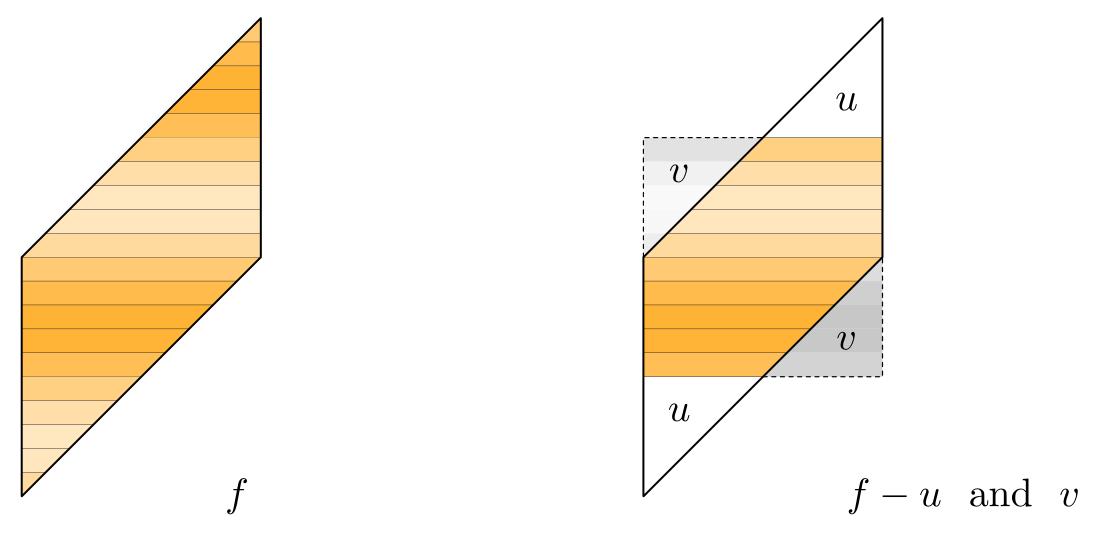
\includegraphics[height=54mm]{SimpleSp.png}
  \end{center}
       
    
\end{frame}



%=================================================================================================
\begin{frame}
  \frametitle{Simplicity of the spectrum}

  Suppose that $\exists\, f_1,f_2$ such that any cyclic space $Z$ contains $g_1,g_2$ 
  satisfying 
  $$
    \|g_1\| = \|g_2\| = a
  $$
  $$
    \frac{\|f_1-g_1\|^2 + \|f_2-g_2\|^2}2 \ge 1+a^2-2a/\sqrt{2} 
  $$
  
  Choose 
  $$
    g_k = \sum_{j=-h_n/2}^{h_n/2} f^{(n)}_k(j) \,{\Hat T}^j b_n
  $$
  
  \medskip
  $$
    g_k = f_k - u_k + v_k
  $$
  
    
\end{frame}



%=================================================================================================
\begin{frame}
  \frametitle{Simplicity of the spectrum}

  {\bf Theorem.} The randomized Salem constructions have simple spectrum.
  
  \bigskip
  {\it Proof.\/} Observe that 
  $$
    \scpr<u,v> \to 0, \qquad \scpr<f,v> \to 0 \qquad \text{as $n \to \infty$}, 
  $$
  and it implies  
  $$
    \|f-g\|^2 \to \frac12, \qquad \|g\| \to \|f\|. 
  $$
    
\end{frame}



%=================================================================================================
\begin{frame}
  \frametitle{Simplicity of the spectrum}

  \begin{center}
  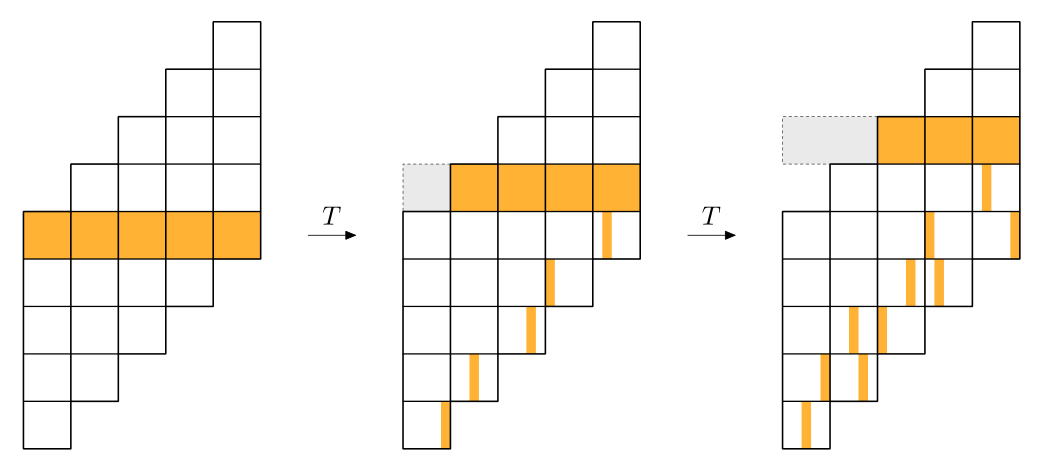
\includegraphics[height=48mm]{SimpleSpDiff.png}
  \end{center}
       
    
\end{frame}



%=================================================================================================
\begin{frame}
  \frametitle{Simplicity of the spectrum}
  
  \begin{align*}
  a^2 &= \|g\|^2 = \|f-u+v\|^2 = \\ 
  &= \|f\|^2 + \|u\|^2 + \|v\|^2 - \\ 
  &\qquad - 2\Re\scpr<f,u> + 2\Re\scpr<f,v> - 2\Re\scpr<u,v> \approx \\
  &\approx \|f\|^2 + 2\|u\|^2 - 2\Re\scpr<f,u> \approx \\ 
  &\approx \|f\|^2 = 1 
  \end{align*}

  % Now let us estimate 
  And the precision of approximation: 
  $$
    \|f-g\|^2 = \|-u+v\|^2 \approx \|u\|^2 + \|v\|^2 \approx \frac12 \|f\|^2 = \frac12. 
  $$

\end{frame}



%=================================================================================================
\begin{frame}
  \frametitle{Simplicity of the spectrum}
  
  \def\qq{\quad  \stackrel{\text{\small ?}}\ge  \quad}

  Having in mind that $a \to 1$ we pass from the inequality 
  $$
    \|f-g\|^2 \qq 1 + a^2 - a\sqrt{2} 
  $$
  to the inequality 
  $$
    \frac12 \qq 2 - \sqrt{2} 
  $$
  $$
    \sqrt{2} {\color{red} \qq} \frac32 
  $$
  which is false. $\Box$ 
  
  \bigskip
  {\bf Phenomenon.} A gap between $\sqrt{2}$ and $3/2$ gives an additional freedom in the construction. 
    
\end{frame}












%~~~~~~~~~~~~~~~~~~~~~~~~~~~~~~~~~~~~~~~~~~~~~~~~~~~~~~~~~~~~~~~~~~~~
\if0=1
\begin{frame}
  \frametitle{SF}

	\medskip	
	\begin{figure}
 		\includegraphics[width=56mm]{specflow1/manif1.pdf} 
	\end{figure}

\end{frame}
\fi
%~~~~~~~~~~~~~~~~~~~~~~~~~~~~~~~~~~~~~~~~~~~~~~~~~~~~~~~~~~~~~~~~~~~~~~~~~~~~




